\newpage

\section*{ $^{45}$Sc(n,$\gamma$)$^{46}$Sc }

Power Level: 100 kW(th) \\
Time at Power: 60.0 m \\
Wait Time:  2.0 d \\
Counting Time: 60.0 m \\
Total Activity at Removal: 4.77e+00 $\mu Ci$

\begin{table*}[h]
\centering
\begin{tabular}{ |c|c|c|c|c|c| }
 \hline
 Position & Mass $mg$ & Counting Activity $\mu Ci$ & Area (Counts) & Error \% \\
 \hline 
 1 & 0.45 & 9.81e-01 & 2.65e+06 & 0.0614 \\ 
\hline
 2 & 0.45 & 1.50e+00 & 4.06e+06 & 0.0496 \\ 
\hline
 3 & 0.45 & 1.39e+00 & 3.77e+06 & 0.0515 \\ 
\hline
 4 & 0.45 & 8.18e-01 & 2.21e+06 & 0.0673 \\ 
\hline
\end{tabular}
\end{table*}

\begin{figure}[h]
\centering
\begin{subfigure}{.5\textwidth}
  \centering
     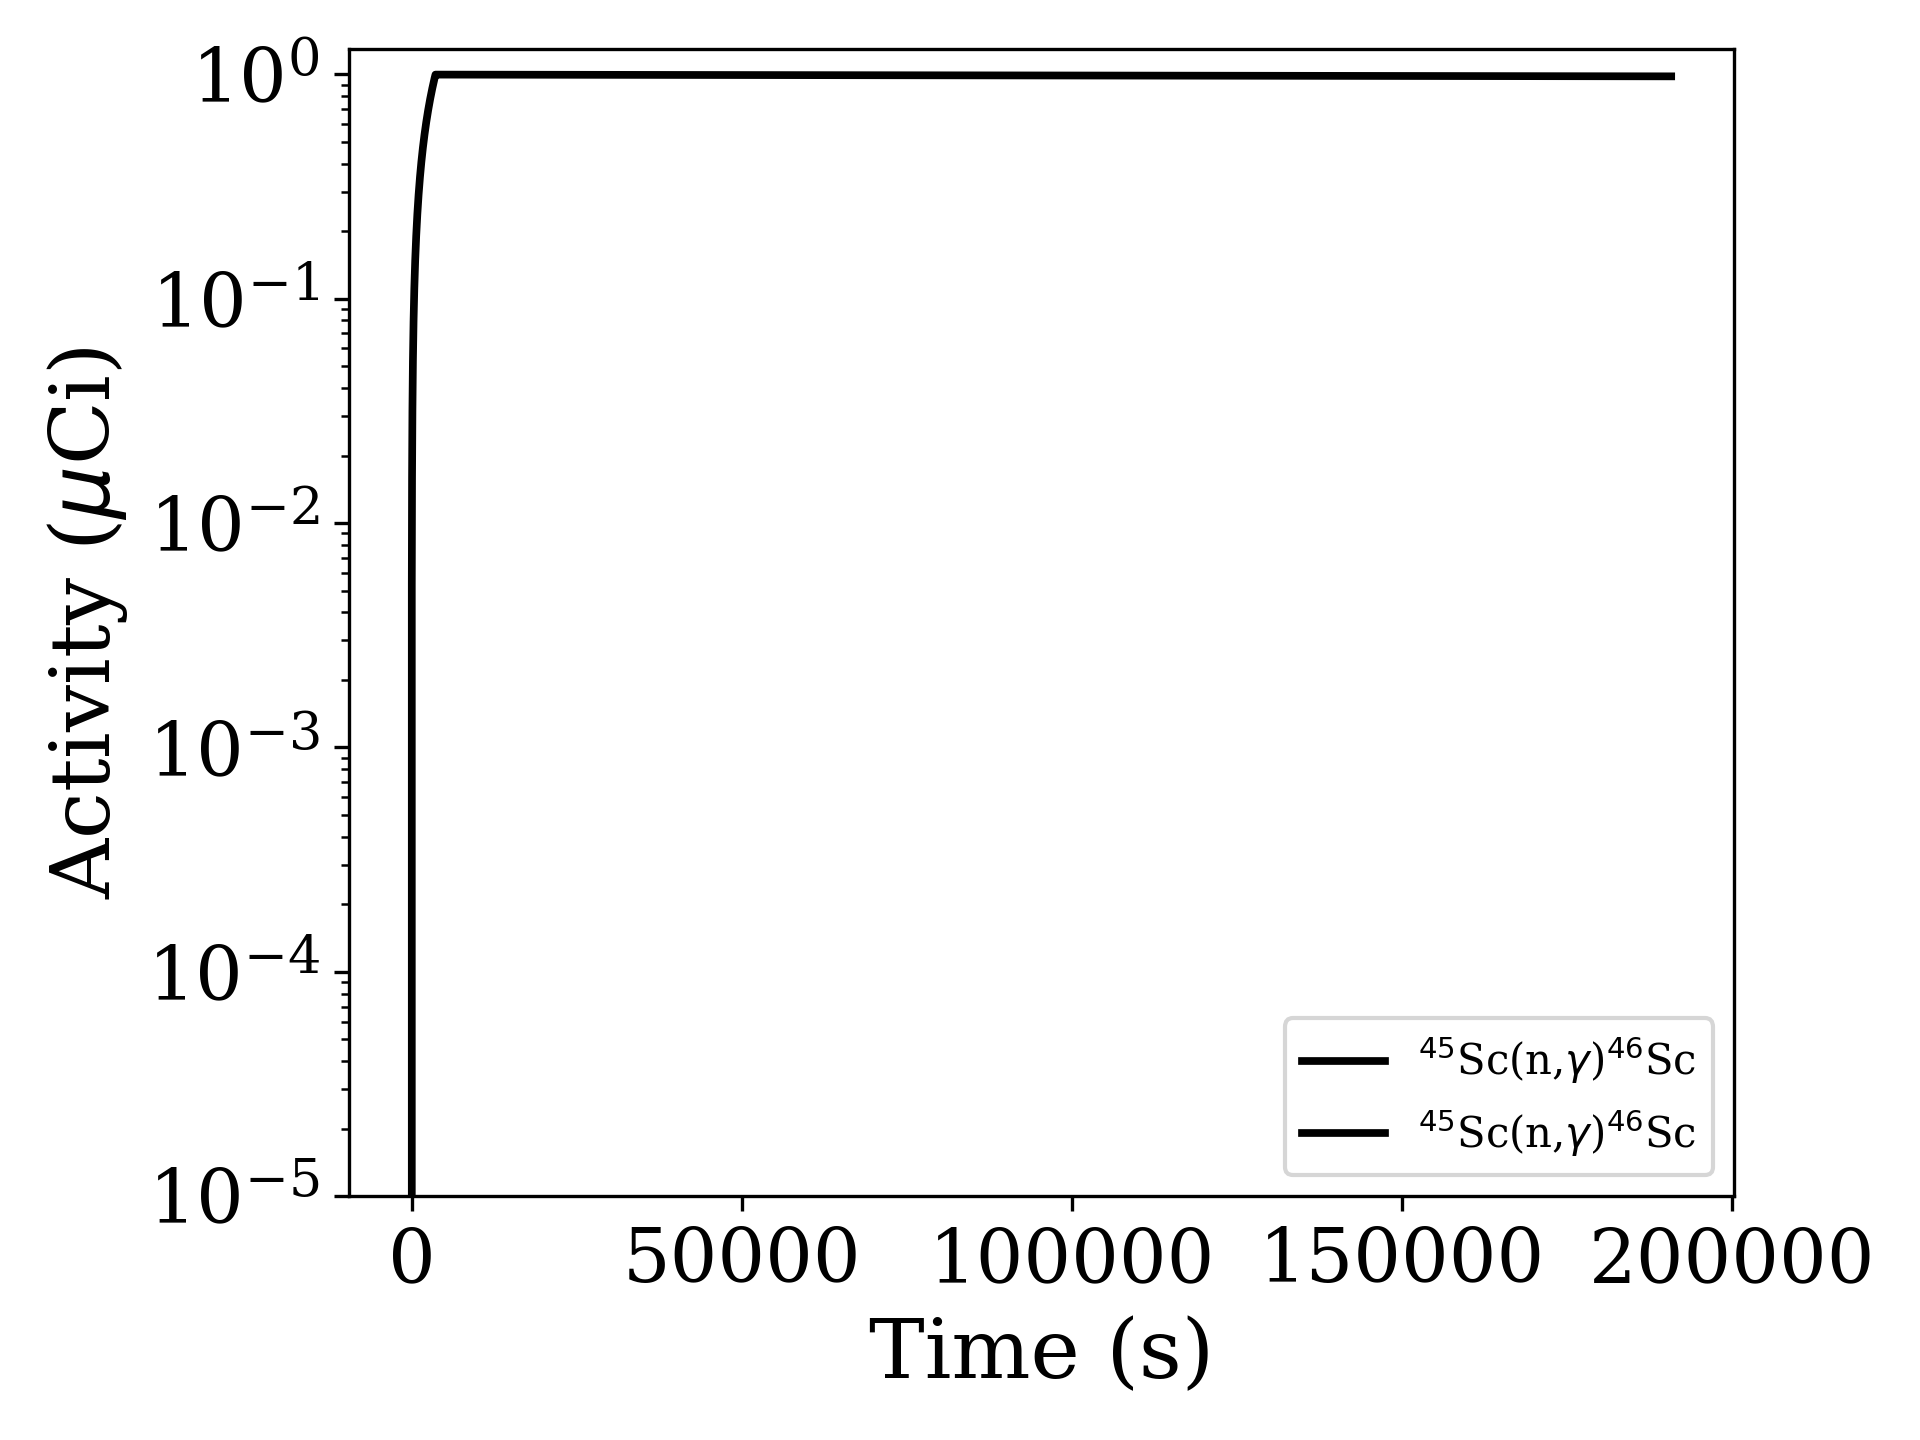
\includegraphics[width=.8\textwidth]{plot/Sc-45(n,gamma)Sc-46_library1} 

  \caption{A subfigure}
  \label{fig:sub1}
\end{subfigure}%
\begin{subfigure}{.5\textwidth}
  \centering
     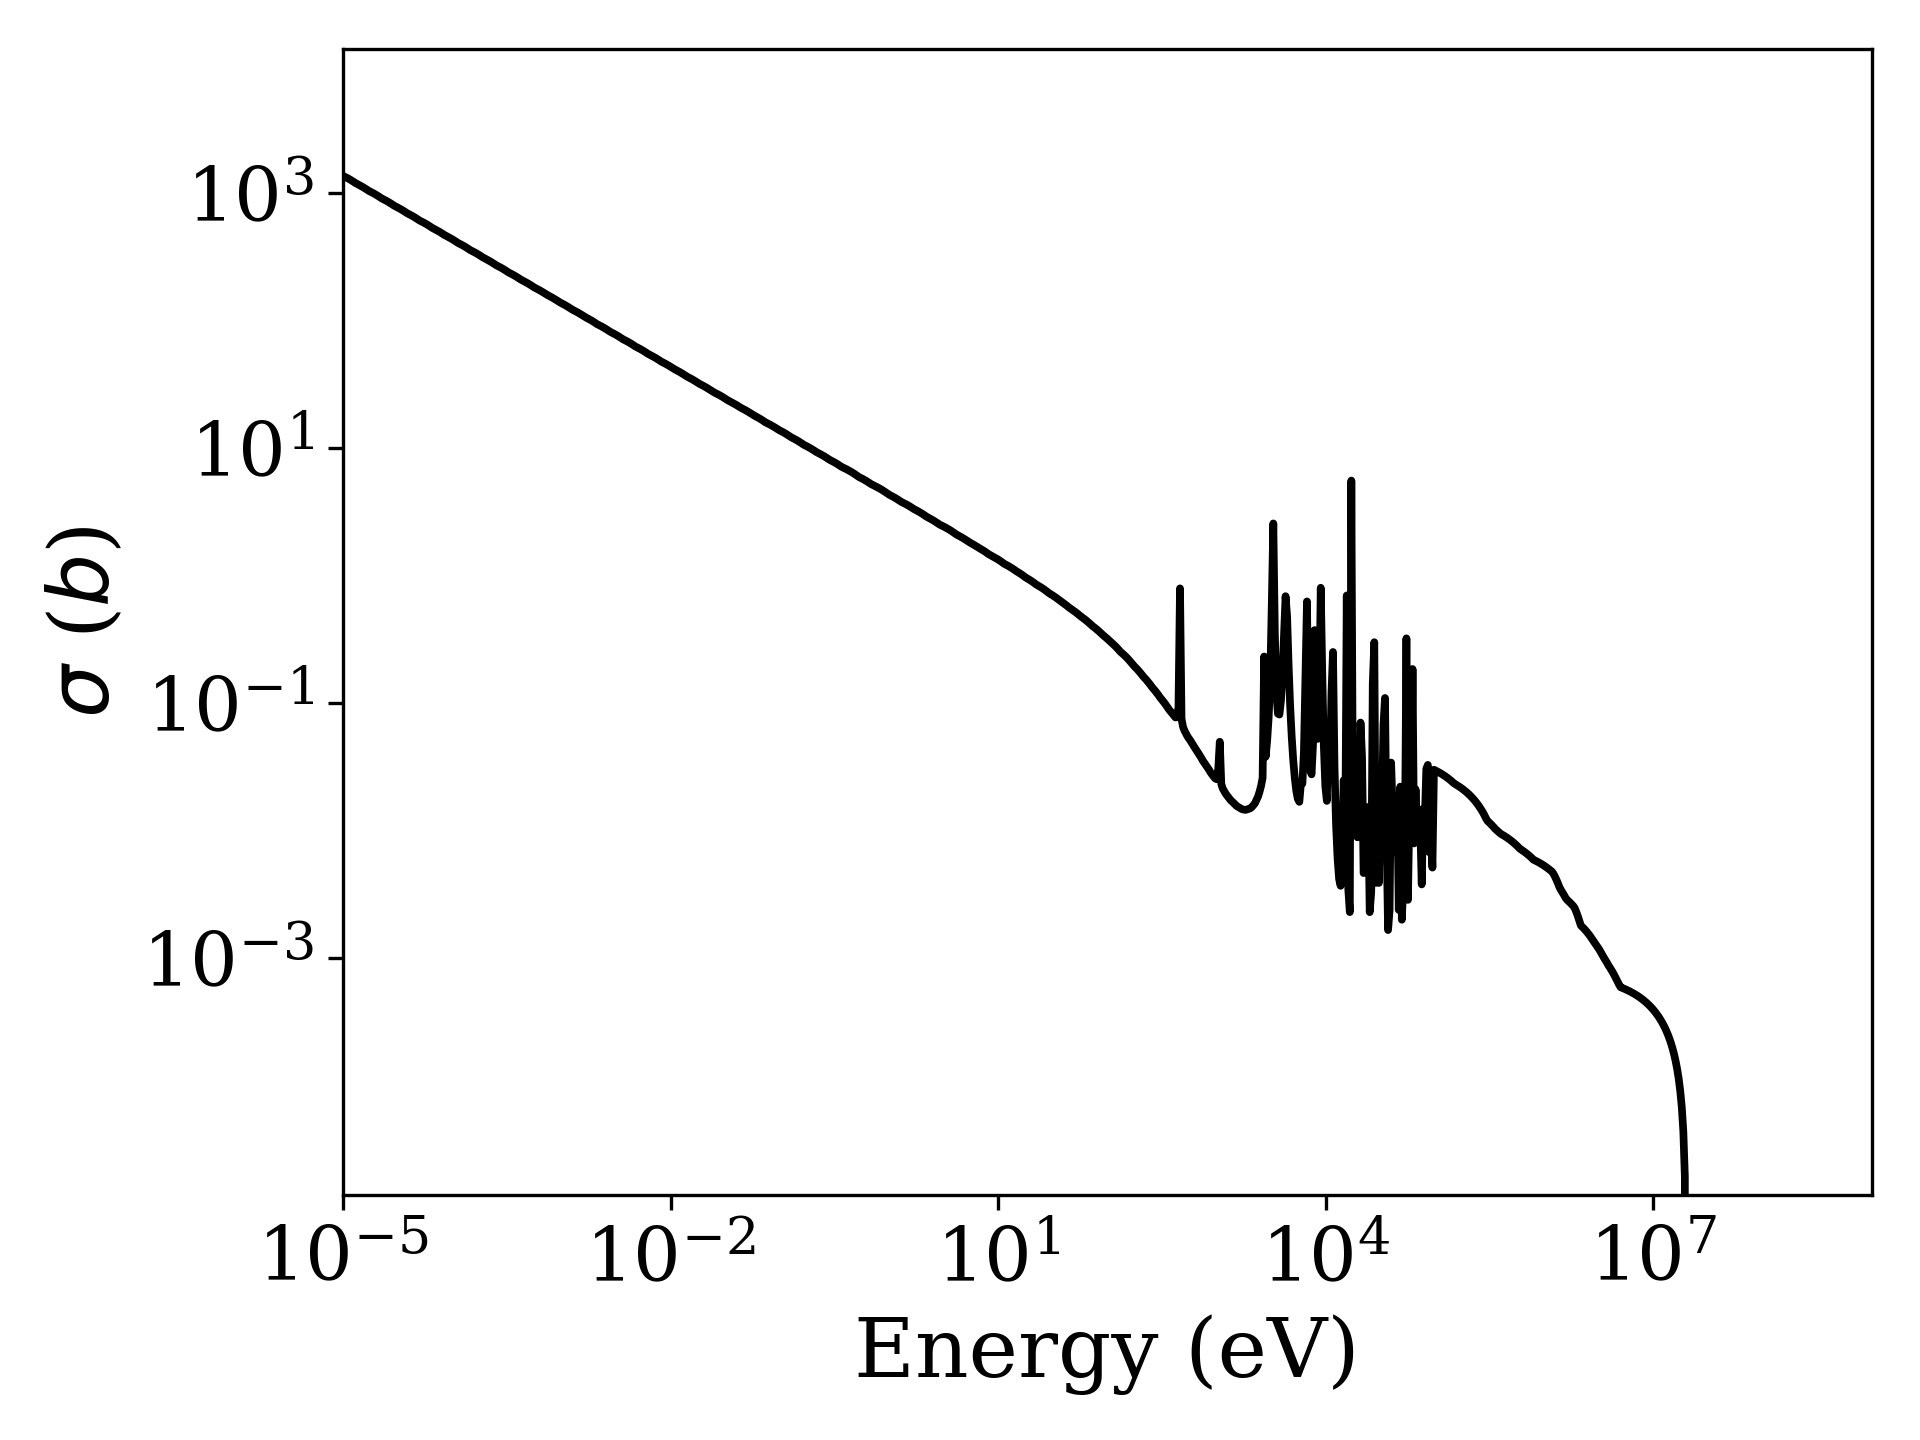
\includegraphics[width=.8\textwidth]{plot/Sc-45(n,gamma)Sc-46} 

  \caption{A subfigure}
  \label{fig:sub2}
\end{subfigure}
\caption{A figure with two subfigures}
\label{fig:test}
\end{figure}

\begin{table*}[h]
\centering
\begin{tabular}{ |c|c|c|c|c|c|c| }
 \hline
 Reaction & T$_{1/2}$ & ROI (eV) & Important Gammas (keV) \\
 \hline 
 $^{45}$Sc(n,$\gamma$)$^{46}$Sc & 84.0 d & 6.66e-03, 5.14e-01 & 1120.545(0.99987) \\ 
\hline
\end{tabular}
\end{table*}
